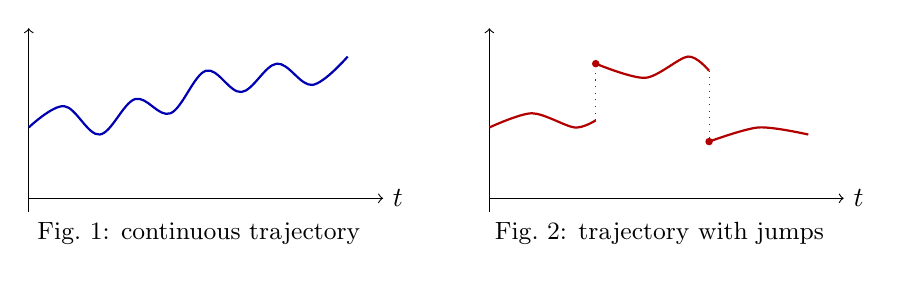
\begin{tikzpicture}[scale=0.9]
\begin{scope}
\draw[->] (0,0)--(5,0) node[right]{$t$}; \draw[->] (0,-0.2)--(0,2.4);
\draw[blue!70!black,thick] plot[smooth,tension=0.6] coordinates {(0,1)(0.5,1.3)(1,0.9)(1.5,1.4)(2,1.2)(2.5,1.8)(3,1.5)(3.5,1.9)(4,1.6)(4.5,2.0)};
\node at (2.4,-0.5) {\small Fig.\ 1: continuous trajectory};
\end{scope}
\begin{scope}[xshift=6.5cm]
\draw[->] (0,0)--(5,0) node[right]{$t$}; \draw[->] (0,-0.2)--(0,2.4);
\draw[red!70!black,thick] plot[smooth] coordinates {(0,1)(0.6,1.2)(1.2,1.0)(1.5,1.1)};
\draw[red!70!black,thick] plot[smooth] coordinates {(1.5,1.9)(2.2,1.7)(2.8,2.0)(3.1,1.8)};
\draw[red!70!black,thick] plot[smooth] coordinates {(3.1,0.8)(3.8,1.0)(4.5,0.9)};
\draw[red!70!black,dotted] (1.5,1.1)--(1.5,1.9); \draw[red!70!black,dotted] (3.1,1.8)--(3.1,0.8);
\fill[red!70!black] (1.5,1.9) circle (1.5pt); \fill[red!70!black] (3.1,0.8) circle (1.5pt);
\node at (2.4,-0.5) {\small Fig.\ 2: trajectory with jumps};
\end{scope}
\end{tikzpicture}
